\section{Grenzwerte und Konvergenz}



\begin{KR}{Grenzwert Berechnen Tricks}
    \begin{itemize}
      \item " $\frac{\infty}{\infty} "$ Trick: Erweitern mit $\frac{1}{n^{k}}$ (k: grösster Exponent)
    \end{itemize}
    
    $\lim _{n \rightarrow \infty} \frac{2 n^{6}-n^{3}}{7 n^{6}+n^{5}-3} \cdot \frac{\frac{1}{n^{6}}}{\frac{1}{n^{6}}}=\frac{2}{7}$
    
    \begin{itemize}
      \item " $\frac{\infty}{\infty} "$ Trick: Erweitern mit $\frac{1}{a^{k}}$ (a: grösste Basis, k: kleinster Exponent) $\lim _{n \rightarrow \infty} \frac{7^{n-1}+2^{n+1}}{7^{n}+5} \cdot \frac{\frac{1}{7^{n-1}}}{\frac{1}{7^{n-1}}}=\frac{1}{7}$
      \item " $\infty-\infty$ " Trick: Erweitern mit $\sqrt{\cdots}+\sqrt{\cdots}$
    \end{itemize}
    
    $\lim _{n \rightarrow \infty}\left(\sqrt{n^{2}+n}-\sqrt{n^{2}+1}\right)=1 / 2$
    
    \begin{itemize}
      \item e-like...: Trick: umformen zu $\left(\left(1+\frac{1}{x}\right)^{x}\right)^{a} \Rightarrow e^{a}$
    \end{itemize}
    \end{KR}

    \begin{concept}{Rechnen mit Grenzwerten von Funktionen}
        \begin{itemize}
            \item $\lim_{x \to x_0} (f + g)(x) = \lim_{x \to x_0} f(x) + \lim_{x \to x_0} g(x)$
            \item $\lim_{x \to x_0} (f \cdot g)(x) = \lim_{x \to x_0} f(x) \cdot \lim_{x \to x_0} g(x)$
            \item Sei $f \leq g$, so ist $\lim_{x \to x_0} f(x) \leq \lim_{x \to x_0} g(x)$
            \item Falls $g_1 \leq f \leq g_2$ und $\lim_{x \to x_0} g_1(x) = \lim_{x \to x_0} g_2(x)$, so existiert $\lim_{x \to x_0} f(x) = \lim_{x \to x_0} g_1(x)$
        \end{itemize}
    \end{concept}

    \begin{formula}{Spezielle Grenzwerte}
        \textcolor{pink}{\[n\rightarrow \infty\]}
        \resizebox*{0.9\linewidth}{!}{
        %\def\arraystretch{1.2}
        \begin{tabular}{c|c|c}
            \(\frac{1}{n}\rightarrow 0\)& \(e^n\rightarrow \infty\)&\(\frac{1}{n^k}\rightarrow 0\ \ \forall k\in
            \mathbb{R}^+\)\\
            \hline
            \(c+\frac{1}{n}\rightarrow c\)&\(e^{-n}\rightarrow 0\)&\((1+n)^{\frac{1}{n}}\rightarrow 1\)\\
            \hline
            \(\frac{c\cdot n}{c^n}\rightarrow 0\)&\(\frac{e^n}{n^c}\rightarrow \infty\)&\(\left(1+\frac{1}{n}\right)^c
            \rightarrow 1\)\\
            \hline
        \(\sqrt[n]{n}=n^{\frac{1}{n}}\rightarrow 1\)&\(\frac{\sin{n}}{n}\rightarrow 0\)&\(\left(1+\frac{1}{n}\right)^n
        \rightarrow e\)\\
        \hline
        \(\sqrt[n]{n!}\rightarrow \infty\)&\(\arctan{n}\rightarrow \frac{\pi}{2}\)&\(\left(1+\frac{c}{n}\right)^n
        \rightarrow e^c\)\\
        \hline
        \(\frac{1}{n}\sqrt[n]{n!} \rightarrow \frac{1}{e}\)&\(\ln{n}\rightarrow \infty\)&\(\left(1-\frac{1}{n} \right)^n
        \rightarrow \frac{1}{e}\)\\
        \hline
        \(\frac{c^n}{n!} \rightarrow 0\)&\(\frac{\ln{n}}{n}\rightarrow 0\)&\(\left(\frac{n}{n+c}\right)^n\rightarrow
        e^{-c}\)\\
        \hline
        \(\frac{n^n}{n!}\rightarrow \infty\)&\(\frac{\log{n}}{n-1}\rightarrow 1\)& \\
        \end{tabular}
        }
        \[n^c\cdot q^n \rightarrow 0 \quad \forall c \in \mathbb{Z},0\leq q \leq 1\]
        \[n(\sqrt[n]{c}-1)\rightarrow \ln{c}\quad \forall c > 0\]
        \textcolor{pink}{\[n\rightarrow 0\]}
        \resizebox*{0.9\linewidth}{!}{
        %\def\arraystretch{1.2}
        \begin{tabular}{c|c|c}
            \(\ln{n}\rightarrow -\infty\)&\(\frac{\sin{n}}{n}\rightarrow 1\)&\(\frac{1}{\arctan{n}}\rightarrow 1\)\\
            \hline
            \(n\log{n}\rightarrow 0\)&\(\frac{\cos{(n)}-1}{n}\rightarrow 0\)&\(\frac{e^n-1}{n}\rightarrow 1\)\\
            \hline
            \(\frac{\log{1}-n}{n}\rightarrow -1\)&\(\frac{1}{\cos{n}}\rightarrow1\)&\(\frac{e^cn-1}{n}\rightarrow c\)\\
            \hline 
            \(\frac{c^n-1}{n}\rightarrow\ln{c},\forall c>0\)&\(\frac{1-\cos{n}}{n^2}\rightarrow
            \frac{1}{2}\)&\((1+n)^{\frac{1}{n}}\rightarrow e\)\\
        \end{tabular}
        }
    \end{formula}

    \begin{definition}{Reihen - Funktionen}\\
        $
        \begin{array}{ll}
            \sum^{n}_{k=1} k = \frac{n \cdot (n+1)}{2} & \sum^{n}_{k=1} (2k - 1)^2 = \frac{n \cdot (4n^2-1)}{3}\\
            \sum^{n}_{k=1} 2k-1 = n^2 & \sum^{n}_{k=1} k^3 = \left( \frac{n \cdot (n+1)}{2}\right)^2\\
            \sum^{n}_{k=1} 2k = n(n+1) & \sum^{n}_{k=1} \frac{1}{k(k+1)} = \frac{n}{n+1}\\
            \sum^{n}_{k=1} k^2 = \frac{n \cdot (n+1) \cdot (2n+2)}{6} &
        \end{array}
        $
    \end{definition}





\subsection{Grenzwerte von Folgen}

\begin{definition}{Formelle Grenzwert Definition}
    Folgende Aussagen sind äquivalent:
    \begin{enumerate}
        \item $\sequence$ konvergiert gegen $l = \lim_{n \to \infty} a_n$
        \item $\forall \varepsilon > 0~\exists N \geq 1$, sodass $|a_n -l | < \varepsilon \quad \forall n \geq N$.
    \end{enumerate}
\end{definition}
Bem: $l$ bezeichnet den Grenzwert $\lim_{n \to \infty} a_n$
\begin{lemma}{Einzigartigkeit Grenzwert}
     Es gibt max. ein $l \in \R$ für $a_n$ mit dieser Eigenschaft (max. 1 Grenzwert)
\end{lemma}
\begin{theorem}{Rechenregeln mit Folgen}
    \\Sei $\sequence,\sequence[b]$ konvergente Folgen mit$a = \lim_{n \to \infty} a_n$, $b = \lim_{n \to \infty} b_n$
    \begin{enumerate}
        \item $(a_n \pm b_n)_{n \geq 1}$ konvergent, $\lim_{n \to \infty} (a_n \pm b_n) = a \pm b$.
        \item $(a_n \cdot b_n)_{n \geq 1}$ konvergent, $\lim_{n \to \infty} (a_n \cdot b_n) = a \cdot b$.
        \item $(a_n \div  b_n)_{n \geq 1}$ konvergent, $\lim_{n \to \infty} (a_n \div b_n) = a \div b$.
        \\(solange $b_n \neq 0 ~ \forall n \geq 1$ und $b \neq 0$)
        \item Falls $\exists K \geq 1$ mit $a_n \leq b_n ~ \forall n \geq K$ folgt $a \leq b$.
    \end{enumerate}
\end{theorem}

\begin{KR}{Konvergenz Folgen}
    \begin{enumerate}
        \item Für Brüche, grösste Potenz von n ausklammern und kürzen. Alle übrigen Brüche der Form $\frac{a}{n^s}$ streichen, da diese zu 0 konvergieren.
        \item Für Wurzeln in einer Summe, multipliziere mit der Differenz der Summe (bei a + b multipliziere mit a - b)
        \item Anwendung Satz von Weierstrass/Sandwich-Satz 
        \item Vergleich mit Referenz-Folgen (Spezielle Grenzwerte)
        \item Umformen/Tricks
        \item Definition der Konvergenz/Limes anwenden
        \item Suchen eines konvergenten Majoranten
    \end{enumerate}
\end{KR}
\begin{KR}{Divergenz Folgen}
    \begin{enumerate}
        \item  Suche einen divergenten Minoranten
        \item Für alternierende Folgen zeige, dass \\$\lim_{n \to \infty} a_p1(n) \neq \lim_{n \to \infty} a_p2(n)$
    \end{enumerate}
\end{KR}



\begin{concept}{Satz von Weierstrass}
    \begin{itemize}
        \item $\sequence$ monoton wachsend und nach oben beschränkt. $\Rightarrow$ $\sequence$ konvergiert mit $\lim_{n \to \infty} a_n = \sup \{a_n : n \geq 1\}$
        \item $\sequence$ monoton fallend und nach unten beschränkt. $\Rightarrow$ $\sequence$ konvergiert mit $\lim_{n \to \infty} a_n = \inf \{a_n : n \geq 1\}$
    \end{itemize}
\end{concept}

\begin{theorem}{Sandwich-Satz}
    Sei $\lim a_n = \alpha$ und $\lim c_n = \alpha$ und $a_n \leq b_n \leq c_n, \forall n \geq k$ dann gilt $\lim b_n = \alpha$\\
    Bmk: k steht hier für eine beliebige natürliche Zahl, ab der die Bedingung immer gilt. Also wie bei der Grenzwert-Definition mit dem <<Gürtel>> um den Grenzwert - das gilt ja auch erst ab einem gewissen Wert n.\\
    Bmk 2: Einfach gesagt heisst das, dass wenn wir den Grenzwert von zwei Folgen bereits kennen und dieser für beide gleich ist, und wir eine dritte Folge haben die <<zwischen>> die zwei bekannten Folgen passt (daher Sandwich-Satz), wissen wir dass auch die dritte Folge den gleichen Grenzwert wie die anderen zwei hat.
\end{theorem}    

\begin{KR}{Binom Trick}\\
    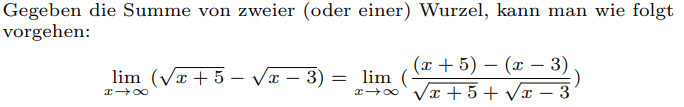
\includegraphics[scale=0.5]{binomtrick.png}
\end{KR}
\begin{KR}{Substitutions Trick}\\
    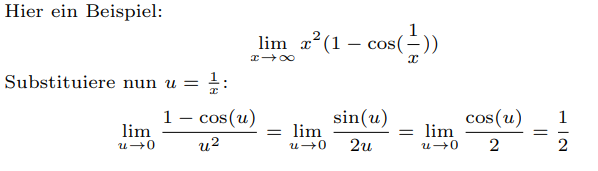
\includegraphics[scale=0.5]{substitutionstrick.png}
\end{KR}


\subsection{Grenzwerte von Reihen}

\begin{concept} {Nullfolgenkriterium}\\
    $\sum_{k=1}^\infty a_k~\text{konvergiert} \Rightarrow \lim_{k \to \infty} a_k = 0$ aber die Umkehrung stimmt nicht.
\end{concept}
\begin{concept} {Cauchy Kriterium}\\
    Die Reihe $\sum_{k=1}^\infty a_k$ ist genau dann konvergent, falls:\\
    $\forall \varepsilon > 0 ~\exists N \geq 1$ mit $\left|\sum_{k=n}^m a_k \right| < \varepsilon \quad \forall m \geq n \geq N$
\end{concept}
\begin{concept} {Leibniz Kriterium}\\
    Sei $\sequence$ monoton fallend, mit $a_n \geq 0~\forall n \geq 1$ und $\lim_{n \to \infty} a_n = 0$. Dann konvergiert\\
    $S \coloneqq \sum_{k = 1}^{\infty} (-1)^{k+1} a_k$
    und es gilt: $a_1 - a_2 \leq S \leq a_1$.
\end{concept}
\begin{concept} {Majorantenkriterium}\\
    Seien $a_n, b_n \geq 0$ mit $a_n \geq b_n \quad \forall n > n_0$:\\
    $\sum_{n=0}^\infty a_n$ konvergiert $\Rightarrow \sum_{n=0}^\infty b_n$ konvergiert 
\end{concept}
\begin{concept} {Minorantenkriterium}\\
    Seien $a_n, b_n \geq 0$ mit $a_n \leq b_n \quad \forall n > n_0$:\\
    $\sum_{n=0}^\infty a_n$ divergiert $\Rightarrow \sum_{n=0}^\infty b_n$ divergiert 
\end{concept}
\begin{concept} {Quotientenkriterium}\\
    Sei $\sequence$ mit $a_n \neq 0~\forall n \geq 1$ und: $q = \frac{|a_{n + 1}|}{|a_n|}$\\
    Falls:
    \begin{itemize}
        \item $q < 1$ konvergiert $\sum_{n=1}^\infty a_n$ absolut
        \item $q > 1$ divergiert $\sum_{n=1}^\infty a_n$
    \end{itemize}
    Für $\liminf a_n = 1$ keine Aussage möglich\\
    \emph{!!! für die harmonische Reihe ist dieses Kriterium nicht anwendbar/gültig !!!}
\end{concept}
\begin{concept} {Wurzelkriterium}\\
    Es sei: $q = \sqrt[n]{|a_n|}$\\
    Dann gilt:
    \begin{itemize}
        \item $q < 1 \Rightarrow \sum_{n=1}^\infty a_n$ konvergiert 
        \item $q > 1 \Rightarrow \sum_{n=1}^\infty a_n$ und $\sum_{n=1}^\infty |a_n|$ divergieren
        \item $q = 1 \Rightarrow$ keine Aussage möglich
    \end{itemize}
\end{concept}
\begin{KR}{Logarithmus abschätzen}\\
    $\log_b (n)$ kann mit $n^\alpha$ ($\alpha > 0$) abgeschätzt werden.\\
    $\ln(n) \leq \sqrt{n}$
\end{KR} 

\raggedcolumns
\columnbreak

\subsection{Funktionen}

\begin{center}
    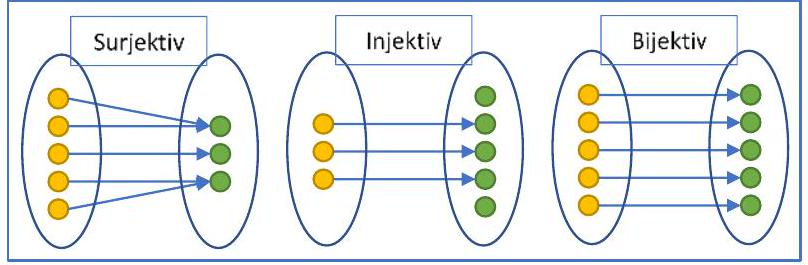
\includegraphics[scale=0.2]{2024_01_20_7bfda6c084929ccc01ffg-01(3).jpg}
\end{center}


\begin{definition}{Umkehrfunktion}
\begin{itemize}
  \item Bijektive Funktion $f: D \rightarrow W$
  \item Umkehrunktion $f^{-1} \quad g: W \rightarrow D$
\end{itemize}
Vorgehen $f(x)=y$:
\begin{itemize}
  \item Nach $x$ auflösen $\quad \rightarrow x=g(y)$
  \item Variablen vertauschen $\rightarrow y=g(x)$
\end{itemize}
\end{definition}



\begin{theorem}{Operationen von Funktionen}
    \begin{itemize}
  \item Addition $x \rightarrow f(x)+g(x)$
  \item Subtraktion $x \rightarrow f(x)-g(x)$
  \item Multiplikation $x \rightarrow f(x) \cdot g(x)$
    \item Division $x \rightarrow f(x) / g(x)$
\end{itemize}



\begin{itemize}
  \item Komposition/Verkettung: $(g \circ f)(x)=g(f(x))$
\end{itemize}
\end{theorem}

\begin{definition}{Symmetrie}
\begin{itemize}
  \item gerade $f(-x)=f(x)$
  \item ungerade $f(-x)=-f(x)$
\end{itemize}
\end{definition}

\begin{center}
    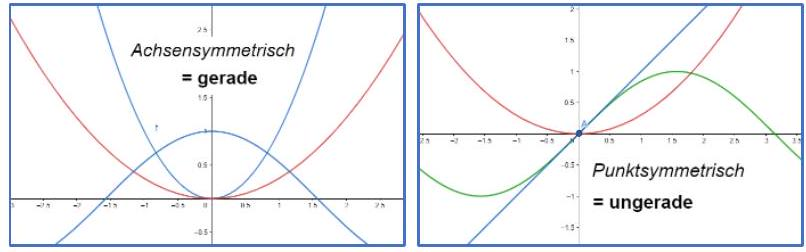
\includegraphics[scale=0.3]{2024_01_20_7bfda6c084929ccc01ffg-01(2).jpg}
\end{center}

\begin{definition}{Beschränktheit}
    Sei $f \in \R^D$.
    \begin{enumerate}
        \item $f$ ist \emph{nach oben beschränkt}, falls $f(D) \subseteq \R$ nach oben beschränkt.
        \item $f$ ist \emph{nach unten beschränkt}, falls $f(D) \subseteq \R$ nach unten beschränkt.
        \item $f$ ist \emph{beschränkt}, falls $f(D) \subseteq \R$ beschränkt.
    \end{enumerate}
\end{definition}

\begin{definition}{Monotonie}
    \begin{itemize}
  \item monoton wachsend $f\left(x_{1}\right) \leq f\left(x_{2}\right)$
  \item streng monoton wachsend $f\left(x_{1}\right)<f\left(x_{2}\right)$
  \item monoton fallend $f\left(x_{1}\right) \geq f\left(x_{2}\right)$
  \item streng monoton wachsend $f\left(x_{1}\right)>f\left(x_{2}\right)$
\end{itemize}
\end{definition}


\begin{definition}{Stetigkeit}
    Eine Funktion ist stetig, falls

    \begin{itemize}
      \item die Kurve keine Sprünge macht
      \item man den Graphen der Funktion zeichnen kann, ohne den Stift dabei abzusetzen
    \end{itemize}

\end{definition}

\begin{formula}{Spezielle Stetige Funktionen}
    \begin{enumerate}
        \item $|f|$, $max(f, g)$ und $min(f, g)$ sind stetig
        \item Polynomielle Funktionen sind auf ganz $\R$ stetig
        \item die Trigonometrischen Funktionen $sin : \R \to \R$ und $cos : \R \to \R$ sind stetig
        \item die Exponentialfunktion $e^x$ ist auf ganz $\R$ stetig
    \end{enumerate}
\end{formula}


\noindent Für mehr wichtige/spezielle Grenzwerte, siehe Grenzwerte von Folgen.
\begin{highlight}{Wichtige Grenzwerte}
    \begin{center}
        \begin{minipage}{0.4\linewidth}
                \tcbsubtitle{Harmonische Folge:}
                $$\lim _{n \rightarrow \infty} \frac{1}{n}=0$$
                \tcbsubtitle{Geometrische Folge:}
                $$\lim _{n \rightarrow \infty} q^n=0 \quad(q<1)$$
        \end{minipage}
        \hfill\vline\hfill
        \begin{minipage}{0.5\linewidth}
            \tcbsubtitle{n-te Wurzel:}
            $$\lim _{n \rightarrow \infty} \sqrt[n]{a}=1$$
            \tcbsubtitle{Eulerzahl:}
            $$\lim _{n \rightarrow \infty}\left(1+\frac{1}{n}\right)^n=e$$
        \end{minipage}
    \end{center}
\end{highlight}

\begin{definition}{Konvergenz einer Funktion}\\
    Die Funktion $y = f(x)$ hat an der Stelle $x_0$ den Grenzwert $y_0$ falls:\\
    für jede Folge $\left(x_{n}\right)$ mit $\lim _{n \rightarrow \infty} x_{n}=x_{0}$ gilt $\lim _{n \rightarrow \infty} f\left(x_{n}\right)=y_{0}$\\
    Bmk: Die Stelle $x_{0}$ muss nicht im Definitionsbereich $D$ sein.
\end{definition}

\begin{definition}{Konvergenz/Divergenz}
    \begin{itemize}
  \item Konvergenz:
  Funktion mit Grenzwert $x \rightarrow \infty$
  \item Divergenz:
  Funktion ohne Grenzwert $x \rightarrow \infty$
  \item Bestimmte Divergenz:
  Funktion mit $\lim _{x \rightarrow \infty} f(x)= \pm \infty$
\end{itemize}
\end{definition}

\begin{definition}{Links- und Rechtsseitige Grenzwerte}\\
    Sei $f : D \to \R$ und $x_0 \in \R$. Wir nehmen an, $x_0$ ist ein Häufungspunkt.\\ Was vereinfacht heisst, dass die Funktion an dieser Stelle evtl. einen Sprung macht, da sich z.B. die Definition ändert. Beispiel:
    \begin{equation*}
            f(x) = \begin{cases}
                0 & x < 0\\
                1 & x \geq 0
            \end{cases}
        \end{equation*}
    Setze in diesem Beispiel $x_0 = 0$, und prüfe ob sich die Funktion von rechts und links dem selben Wert nähert bei $x_0$. (NEIN in diesem Bsp.)

    \emph{Formell:} Eine Funktion ist dann gleichmässig konvergent wenn für alle Werte der Funktion gilt

    $$\lim_{x \to x_0^+} f(x) = \lim_{x \to x_0^-} f(x)$$

    (Linksseitiger Grenzwert = Rechtsseitiger Grenzwert)
\end{definition}

\begin{corollary}{Rechnen mit Grenzwerten von Funktionen}
    \begin{itemize}
        \item $\lim_{x \to x_0} (f + g)(x) = \lim_{x \to x_0} f(x) + \lim_{x \to x_0} g(x)$
        \item $\lim_{x \to x_0} (f \cdot g)(x) = \lim_{x \to x_0} f(x) \cdot \lim_{x \to x_0} g(x)$
        \item Sei $f \leq g$, so ist $\lim_{x \to x_0} f(x) \leq \lim_{x \to x_0} g(x)$
        \item Falls $g_1 \leq f \leq g_2$ und $\lim_{x \to x_0} g_1(x) = \lim_{x \to x_0} g_2(x)$, so existiert $\lim_{x \to x_0} f(x) = \lim_{x \to x_0} g_1(x)$
    \end{itemize}
\end{corollary}

\begin{concept}{l'Hospital Kettenregel Trick}
    Seien $f,g : ]a,b[ \to \R$ differenzierbar mit \\ $g'(x) \neq 0 \quad \forall x \in ]a,b[$. Falls $\lim_{x \to b^-} f(x) = 0$, $\lim_{x \to b^-} g(x) = 0$ und $\lambda \coloneqq \lim_{x \to b^-} \frac{f'(x)}{g'(x)}$ existiert, folgt
    \begin{iequation}
        \lim_{x \to b^-} \frac{f(x)}{g(x)} = \lim_{x \to b^-}\frac{f'(x)}{g'(x)}
    \end{iequation}
    \tcblower
    \emph{Nur für $\lim_{x \to 0} \frac{f(x)}{g(x)} = \frac{\mlqq 0 \mrqq}{\mlqq 0 \mrqq}$ oder $\frac{\mlqq \infty \mrqq}{\mlqq \infty \mrqq}$ erlaubt.}
\end{concept}

\raggedcolumns
\pagebreak

\section{Taylorrreihen}

\begin{definition}{Potenzreihe} undendliche Reihe vom Typ:
    \begin{center}
    $p(x)=a_0+a_1x+a_2x^2+ \cdots = \sum_{k=0}^{\infty}{a_kx^k} $\\
    \vspace{2mm}
    \(a_0,a_1, \cdots \in \R\) sind die Koeffizienten der Potenzreihe
    \end{center}
    Allgemein kann eine Potenzreihe mit einer Verschiebung von \(x_0\) beschrieben werden $\Rightarrow$ Potenzreihe mit Zentrum \(x_0\):
    \begin{center}
    $p(x)=a_0+a_1(x-x_0)+a_2(x-x_0)^2+\cdots = \sum_{k=0}^{\infty}{a_k(x-x_0)^k}$
    \end{center}
\end{definition}

\begin{definition}{Taylorreihe} oder Taylorentwicklung einer Funktion \(y=f(x)\) and der Stelle \(x_0\) ist die Potenzreihe:
  \begin{center}
    $t_f(x)=\sum_{k=0}^{\infty}{a_k(x-x_0)^k}$
  \end{center}
  welche die gleiche Ableitung an der Stelle \(x_0 \text{ für alle }k\in \mathbb{N}\) hat wie die Funktion \(f(x)\)
\end{definition}

\begin{definition}{Taylorpolynom}
  ist eine Taylorreihe \(t_f(x)\) welche nach \(n\text{-ter}\) Ordnung abgebrochen wird.
        Somit erhällt man das Taylorpolynom \(n\text{-ter}\) Ordnung von \(f(x)\) an der Stelle \(x_0\):
    \begin{center}
    $p_n(x)=\sum_{k=0}^{n}{a_k(x-x_0)^k}$
    \end{center}
    Bemerkung: Die Tangente der Funktionskurve \(y=f(x) \) an der Stelle \(x_0\) ist exakt das Taylorpolynom 1.
      Ordnung von \(f(x)\) an der Stelle \(x_0\)
\end{definition}

\begin{KR}{Vorgehen Berechnen Taylorreihe}
  Die Taylorreihe einer beliebig oft differenzierbaren Funktion \(t(x)\) an der Stelle \(x_0\) ist:
  \[t_f(x) = \sum_{k=0}^{\infty}{\frac{f^{k}(x_0)}{k!}\cdot(x-x_0)^k}\]
\end{KR}

\begin{formula}{Formel für Taylorkoeffizienten} 
  Formel für \(k\)-ten Taylorkoeffizientn der Taylorreihe \(t_f(x)\) von \(f(x)\) an der Stelle
  \(x_0\in\mathbb{R}\):
  \[a_k=\frac{f^{(k)}(x_0)}{k!}\quad (k\in\mathbb{N})\]
\end{formula}

\begin{theorem}{Taylorreihen wichtiger Funktionen}\\
    \def\arraystretch{2}
  \begin{tabular}{c}
  \(f(x)=e^x \text{ mit }x_0=0,\)\\\(t_f(x)=\sum_{k=0}^{\infty}{\frac{x^k}{k!}}=1+x+\frac{x^2}{2!}+\frac{x^3}{3!}\ldots\)\\
  \hline
  \(f(x)=\sin{(x)}\text{ mit }x_0=0,\)\\\(  t_f(x)=\sum_{k=0}^{\infty}{(-1)^k\frac{x^{2k+1}}{(2k+1)!}}=x-\frac{x^3}{3!}+\frac{x^5}{5!}-\ldots\)\\
  \hline
  \(f(x)=\cos{(x)}\text{ mit }x_0=0,\)\\\(
  t_f(x)=\sum_{k=0}^{\infty}{(-1)^k\frac{x^{2k}}{(2k)!}}=1-\frac{x^2}{2!}+\frac{x^4}{4!}-\ldots\)\\
  \hline
  \(f(x)=\ln{(x)}\text{ mit }x_0=1,\)\\\(
  t_f(x)=\sum_{k=1}^{\infty}{\frac{(-1)^{k+1}}{k}(x-1)^k}=(x-1)-\frac{(x-1)^2}{2}+\frac{(x-1)^3}{3}-\ldots\)\\
\end{tabular}
\end{theorem}



\subsubsection{Symmetrie von Potenzreihen und Taylorreihen}
\begin{concept}{Symmetrie von Funktionen Repetition}
  \begin{itemize}
    \item Gerade Funktion: Funktion für die gilt: \(f(-x)=f(x)\) für alle \(x\in\mathbb{R}\rightarrow\) Funktion ist
      achsensymetrisch bzgl. \(y\)-Achse
    \item Ungerade Funktion: Funktion für die gilt: \(f(-x)=-f(x)\) für alle \(x\in\mathbb{R}\rightarrow\) Funktion ist
      punktsymetrisch bzgl. des Ursprungs
  \end{itemize}
\end{concept}

\begin{concept}{Symmetrie von Potenzreihen}
  Eine Potenzreihe
  \[y=\sum_{k=0}^{\infty}{a_kx^k}=a_0+a_1x+a_2x^2+\cdots\]
  ist eine gerade bzw. ungerade Funktion, falls sie nur gerade bzw. nur ungerade Potenzen enthält.
\end{concept}

\begin{concept}{Symmetrie von Taylorreihen}
  \begin{itemize}
    \item  Falls die Funktion eine gerade Funktion ist, enthällt die Taylorreihe von \(f(x)\) an der Stelle \(x_0 = 0\)
      nur Potenzen mit geraden Exponenten,d.h. se gilt \(a_{2k+1}=0\) für alle \(k\in\mathbb{N}\)
    \item  Falls die Funktion eine ungerade Funktion ist, enthällt die Taylorreihe von \(f(x)\) an der Stelle \(x_0 = 0\)
      nur Potenzen mit ungeraden Exponenten,d.h. se gilt \(a_{2k}=0\) für alle \(k\in\mathbb{N}\)
  \end{itemize}
\end{concept}


\subsubsection{Binomialkoeffizienten}
\begin{KR}{Taylorreihen mit Binomialkoeffizienten bestimmen}
  \begin{itemize}
    \item Ziel: Taylorreihe von Potenzen mit beliebigen (nicht-natürlichen) Exponenten bestimmen, d.h. Funktionen vom
      Typ \(f(x=x^{\alpha})\) mit \(\alpha \in \mathbb{R}\)
    \item Untersuchen der Funktion bei \(f(x)=(1+x)^{\alpha}\) an der Stelle \(x_0=0\)
    \item Falls \(\alpha\in\mathbb{N}\) ist \(f(x)=(1+x)^{\alpha}\) ein Polynom (binomische Formel):
      \[(1+x)^n=\sum_{k=0}^n{\begin{pmatrix}n\\k\end{pmatrix}x^k},\quad
      \begin{pmatrix}n\\k\end{pmatrix}=\frac{n!}{k!(n-k)!}\quad (0\le k \le n)\]
    \item In diesem fall ist die binomische Formel auch die Taylorreihe, es gilt:
      \[a_k=\frac{f^{(k)}(0)}{k!}=\begin{pmatrix}n\\k\end{pmatrix}\]
    \item Falls \(\alpha\in\mathbb{R}\):
    \subitem Taylorkoeffizienten:
    \[\frac{f^{(k)}(0)}{k!}=\frac{\alpha\cdot(\alpha -1)\cdot\cdots\cdot(\alpha-k+1)}{k!}= 
      \begin{pmatrix}\alpha\\k\end{pmatrix}\quad (\alpha\in\mathbb{R},k\in\mathbb{N})\]
    \subitem Taylorreihe:
    \[t_f(x)=1+\begin{pmatrix}\alpha\\1\end{pmatrix}x+\begin{pmatrix}\alpha\\2\end{pmatrix}x^2+
    \begin{pmatrix}\alpha\\3\end{pmatrix}x^3+\cdots =\sum_{k=0}^{\infty}{\begin{pmatrix}\alpha\\k\end{pmatrix}x^k}\]
    Auch bekannt als Binomialreihe
  \end{itemize}
\end{KR}

\subsubsection{Konvergenz von Potenzreihen}
\begin{definition}{Konvergenzradius}
  \begin{itemize}
    \item Der Konvergenzradius \(\rho\) einer Potenzreih\\ \(p(x)=\sum_{k=0}^{\infty}{a_k(x-x_0)^k}\) ist
      eine Zahl mit Folgenden Eigenschaften:
      \subitem - Für alle \(x\in\mathbb{R}\) mit \(|x-x_0|<\rho\) konvergiert die Reihe \(p(x)\)
      \subitem - Für alle \(x\in\mathbb{R}\) mit \(|x-x_0|>\rho\) divergiert die Reihe \(p(x)\)
    \item Es existieren folgende Extremfälle:
      \subitem - Konvergenzradius \(\rho = 0\): Dann konvergiert die Reihe \(p(x)\) nur für \(x=x_0\).
      \subitem - Konvergenzradius \(\rho = \infty\): Dann konvergiert die Reihe \(p(x)\) für alle \(x\in\mathbb{R}\).
  \end{itemize}
\end{definition}
\begin{formula}{Konvergenzradius Formel}\\
  Für die Potenzreihe \(\displaystyle p(x)=\sum_{k=0}^{\infty}{a_k(x-x_0)^k} \) ist der Konvergenzradius:
  \[\rho = \underset{k \rightarrow \infty}{\lim}\left| \frac{a_k}{a_{k+1}}\right| \quad \text{oder} \quad
  \rho=\underset{k \rightarrow \infty}{\lim} \frac{1}{\sqrt[k]{|a_k|} }\]
\end{formula}
\begin{formula}{Konvergenzbereich Formel}\\
  Der Konvergenzbereich in dem die Approximation der Funktion gilt ist definiert durch:
  \[(x_0 - \rho , x_0 + \rho) \]
\end{formula}

\subsubsection{Bernuolli- de l'Hospital}
\begin{definition}{Regel von Bernoulli- de l’Hospital}
      Wenn die Funktionen \(f(x)\text{ und }g(x)\) an der Stelle \(x_0\) stetig differenzierbar sind aber der
      Grenzwert auf die Form \(\frac{0}{0}\text{ oder }\frac{\infty}{\infty}\) führt, kann der Limes der Ableitung
      beider Funktionen ausgewerted werden:
      \[\underset{x\rightarrow x_0}\lim\frac{f(x)}{g(x)}=\underset{x\rightarrow x_0}{\lim}\frac{f'(x)}{g'(x)}\]
      Dies kann beliebig oft Wiederholt werden, es gibt jedoch Fälle wo die Regel versagt, dann müssen andere
      Methoden verwendet werden.
\end{definition}

\begin{definition}{Varianten von l'Hospital}\\
  \(\underset{x\rightarrow x_0}{\lim}f(x)\cdot g(x)\) von der Form \(0\cdot \infty\):
  \[f(x)\cdot g(x)=\frac{f(x)}{\frac{1}{g(x)}}\]
  \(\underset{x\rightarrow x_0}{\lim}(f(x)-g(x))\) von der Form \(\infty - \infty\):
  \[f(x)-g(x)=\frac{\frac{1}{g(x)}-\frac{1}{f(x)}}{\frac{1}{f(x)\cdot g(x)}}\]
\end{definition}









